\chapter{二维坐标、时间与接口}\label{ch:frames}
\begin{notebox}
\textbf{目标}\quad 正确旋转、平移、求逆，并用一个仿真时钟驱动坐标树。\\
\textbf{先修}\quad 第 1 章；二维向量和正弦、余弦。矩阵只需要理解本章的两行乘法。
\end{notebox}

\section{一个点可以有不同坐标}
机器人位于地图坐标 $(1,2)$，朝向正北。雷达观测到正前方 2 m 的点。它在机体系是 $(2,0)$，在地图系是 $(1,4)$。坐标变了，物理上的点没有变。

我们采用右手系：机体 x 轴向前、y 轴向左、z 轴向上，逆时针偏航为正，角度使用弧度。一个平面位姿记作 $T_{A\leftarrow B}=(t,\psi)$：它把 B 系的坐标换成 A 系坐标。

\subsection*{从两根坐标轴得到旋转矩阵}
先想象只旋转一个向量，暂时把两个坐标系原点放在一起。
沿 B 系 x 轴走 1 m，在 A 系中的水平、竖直分量分别为 $\cos\psi,\sin\psi$。
B 系 y 轴比 x 轴多转 $\pi/2$，其分量是 $-\sin\psi,\cos\psi$。
任意点 $p_B=(x_B,y_B)$ 都可看成“沿第一根轴走 $x_B$，再沿第二根轴走 $y_B$”，所以
\begin{align}
x_A-t_x&=x_B\cos\psi-y_B\sin\psi,\\
y_A-t_y&=x_B\sin\psi+y_B\cos\psi.
\end{align}
矩阵只是把这两行计算排在一起：第一列记录旋转后的 x 轴，第二列记录旋转后的 y 轴。
向量默认写成一列，上标 $\top$ 表示把行、列互换。
\begin{equation}
R(\psi)=\begin{bmatrix}\cos\psi&-\sin\psi\\ \sin\psi&\cos\psi\end{bmatrix},
\qquad p_A=R(\psi)p_B+t.
\label{eq:transform}
\end{equation}
先旋转向量，再加上 B 原点在 A 中的位置 t。例子中 $\psi=\pi/2$，
$R(2,0)^\top=(0,2)^\top$，再加 $(1,2)^\top$ 就得到 $(1,4)^\top$。
这个顺序对应两件不同的事：坐标轴改变方向，坐标原点改变位置。

\begin{center}
\begin{tikzpicture}[x=1cm,y=1cm,>=Stealth]
\draw[step=1,linecolor] (0,0) grid (4,4);
\draw[->,muted] (0,0)--(4.5,0) node[right] {$x_{\rm map}$};
\draw[->,muted] (0,0)--(0,4.7) node[above] {$y_{\rm map}$};
% 虚线只延长机体 x 轴，不叠画在实线和箭头上。
\draw[dashed,tealblue] (1,3.25)--(1,4);
\draw[tealblue,thick,->] (1,2)--(1,3.2);
\draw[tealblue,thick,->] (1,2)--(.1,2);
\node[right,tealblue,fill=white,inner sep=2pt] at (1.18,3.25) {$x_{\rm body}$};
\node[left,tealblue] at (-.15,2.3) {$y_{\rm body}$};
% 坐标说明放到网格外，用引线指向对应点。
\draw[muted,thin] (1.12,2.03)--(3.5,2.55)--(4.35,2.55);
\node[right,align=left] at (4.45,2.55) {圆心\\map $(1,2)$};
\draw[muted,thin] (1.12,4.07)--(3.5,4.35)--(4.35,4.35);
\node[right,align=left] at (4.45,4.35)
  {同一个观测点\\map $(1,4)$，body $(2,0)$};
\fill[tealblue] (1,2) circle (2pt);
\fill[navy] (1,4) circle (2pt);
\end{tikzpicture}
\end{center}

\section{从公式到一个小函数}
\code{Pose2D} 只保存一个二维向量和一个角度。几何库不包含 ROS 头文件，可以单独用 C++17 编译、调试和测试。
\lstinputlisting[language=C++,linerange={rotation_begin-rotation_end},
  includerangemarker=false]{../ros2_ws/src/motion2d/src/geometry/se2.cpp}

\paragraph{代码中的每一步}
Matrix2d 表示 $2\times2$ 的数表；逗号初始化依次填写两行。
transformPoint 中的矩阵乘法正是上面的两行标量式，pose.position 就是 t。
可以先在纸上算 $\psi=0$ 和 $\psi=\pi/2$，再单步调试查看四个矩阵元素。
函数所在的 se2 文件名表示平面刚体变换；本章所需运算就是旋转、平移与合成。

\section{逆变换与变换链}
从式 \eqref{eq:transform} 两侧减去 t，再左乘 $R^\top$：
\begin{equation}
p_B=R^\top(p_A-t)=R^\top p_A-R^\top t.
\end{equation}
为什么左乘 $R^\top$ 能消去 R？把矩阵直接相乘：
\begin{equation}
R^\top R=
\begin{bmatrix}
\cos^2\psi+\sin^2\psi&-\cos\psi\sin\psi+\sin\psi\cos\psi\\
-\sin\psi\cos\psi+\cos\psi\sin\psi&\sin^2\psi+\cos^2\psi
\end{bmatrix}=I.
\end{equation}
I 是对角线为1、其余为0的单位矩阵，乘向量后保持原值。
因此逆旋转等于转置，逆位姿为 $(-R^\top t,-\psi)$。
手算例子中，先做 $(1,4)-(1,2)=(0,2)$，再顺时针转 $90^\circ$，就回到 $(2,0)$。

若雷达相对机体有固定外参 $T_{B\leftarrow L}$，机体相对地图为 $T_{M\leftarrow B}$，则
\begin{equation}
T_{M\leftarrow L}=T_{M\leftarrow B}T_{B\leftarrow L}.
\end{equation}
这里的位姿乘号表示“接着做另一个变换”。写出中间点便能展开它：
\begin{align}
p_B&=R_{BL}p_L+t_{BL},\\
p_M&=R_{MB}(R_{BL}p_L+t_{BL})+t_{MB}\\
   &=(R_{MB}R_{BL})p_L+(R_{MB}t_{BL}+t_{MB}).
\end{align}
所以合成的平移为 $R_{MB}t_{BL}+t_{MB}$，朝向为 $\psi_{MB}+\psi_{BL}$。
compose 正是先调用 transformPoint 得到这个平移，再相加朝向。
例如雷达在车体前方0.5 m，车体位于 $(1,2)$ 且朝北，雷达在地图中就位于 $(1,2.5)$。
从右向左读下标，便得到“雷达点→机体点→地图点”的计算顺序。课程默认传感器位于圆心，外参为单位变换；保留显式外参能让后续实验改变安装位置。

\section{运行与理解数值误差}
按第 1 章的方法重新构建、加载环境，在工作空间运行：
\begin{lstlisting}[language=bash,numbers=none]
ros2 run motion2d se2_demo
colcon test --packages-select motion2d \
  --event-handlers console_direct+
colcon test-result --verbose
\end{lstlisting}
示例输出机体点 $(2,0)$、地图点 $(1,4)$，再恢复到 $(2,0)$。
浮点运算中的 $\cos(\pi/2)$ 可能是接近零的小数，所以比较使用绝对误差容限 $10^{-12}$，不是要求每个计算结果逐位相同。

角度是另一个边界问题。$179^\circ$ 到 $-179^\circ$ 的最短旋转只有 $2^\circ$。先将差值归一到 $[-\pi,\pi)$，再把它作为误差。函数 \code{wrapAngle} 使用弧度；输入 90 表示 90 rad，不是 90 度。

\section{练习：自己写一次逆变换}
\begin{enumerate}
\item \textbf{推导：}为何逆变换中不能只把 t 取负？用 $\psi=90^\circ,t=(1,2)$ 给一个反例。
\item \textbf{代码：}补完 \path{exercises/ch02/starter/inverse_point.hpp} 的标记函数。它复用正式库的 \code{Pose2D}，检查包括两个旋转方向。
\item \textbf{实验：}把示例朝向换成 $-90^\circ$，预测地图点，再运行核对。还可以将激光外参设为机体前方 0.5 m，手算其地图位置。
\end{enumerate}
独立编译命令、分级提示和参考答案位于同章习题 README。用正向变换再逆变换的往返结果检查自己：应回到原来的点，差别只剩浮点舍入误差。

\section{仿真时间与真实等待时间}
假设每个仿真步长是 $\Delta t=0.005$ s。第 k 步的仿真时间为
\begin{equation}
t_k=k\Delta t.
\end{equation}
即使电脑偶尔调度得慢，状态仍然只前进一个固定步长。例如电脑用0.008 s才完成一次计算，模拟时刻仍从0.005 s增加到0.010 s；
真实等待时间决定程序跑得快慢，仿真时间决定方程积分了多久。

\code{SimClock} 用整数 tick 和整数纳秒保存时间，避免反复执行浮点加法。暂停时自动 advance 返回 false，单步只在暂停时允许执行：
\par\noindent\begin{minipage}{\linewidth}
\lstinputlisting[language=C++,linerange={clock_begin-clock_end},
  includerangemarker=false]{../ros2_ws/src/motion2d/src/sim/sim_clock.cpp}
\end{minipage}\par
本章由 \code{frame_demo_node} 唯一发布 \code{/clock}；RViz2 和节点都设置 \code{use_sim_time=true}。
暂停后重复发送当前时间，便于新订阅者获得它。判断是否发生新的一步，应比较时间值，而不是数消息。
例如收到0.010、0.010、0.015 s三条消息，物理状态只从第2步推进到第3步。

\section{把坐标放到 ROS 的 TF 树中}
\[
\texttt{map}\to\texttt{odom}\to\texttt{base\_link}
\to\{\texttt{laser},\texttt{imu\_link}\}.
\]
本章 map 到 odom 为单位变换；传感器位于圆心、与机体系对齐，也是单位变换。这三条静态边通过 \code{/tf_static} 发布。odom 到 base\_link 是带采样时刻的动态边，通过 \code{/tf} 发布。

为观察旋转效果，示例固定圆心 $(1,2)$，采用解析朝向
\begin{equation}
\psi(t)=\frac{\pi}{2}+0.2t.
\end{equation}
角速度由求导得到 $\dot\psi=0.2$ rad/s。圆心固定、坐标轴匀速转动，
因此图中的蓝色箭头能清楚展示同一个 laser 系向量怎样在地图中转动。

\subsection*{消息里为什么出现半角？}
ROS 用四个数表示空间朝向。本课程只有绕 z 轴的平面旋转，令 $q_x=q_y=0$。
接口的平面旋转关系为
\begin{equation}
R_q=\begin{bmatrix}1-2q_z^2&-2q_zq_w\\2q_zq_w&1-2q_z^2\end{bmatrix},
\qquad q_z^2+q_w^2=1.
\end{equation}
用一个角 $\theta$ 参数化单位圆：$q_z=\sin\theta,q_w=\cos\theta$。
双角公式给出 $1-2\sin^2\theta=\cos2\theta$、$2\sin\theta\cos\theta=\sin2\theta$，
因此 $R_q=R(2\theta)$。为了表示 yaw=$\psi$，应取 $\theta=\psi/2$：
\begin{equation}
(q_x,q_y,q_z,q_w)=(0,0,\sin(\psi/2),\cos(\psi/2)).
\end{equation}
例如 $90^\circ$ 对应 $q_z=q_w=\sqrt2/2$；零角对应 $(0,0,0,1)$。
这也解释了第一章为什么把 w 设为1：它满足单位长度并表示零旋转。
发布时刻直接取仿真时钟，不能换成回调到达的真实时间：
\par\noindent\begin{minipage}{\linewidth}
\lstinputlisting[language=C++,linerange={frame_begin-frame_end},
  includerangemarker=false]{../ros2_ws/src/motion2d/src/nodes/frame_demo_node.cpp}
\end{minipage}\par

\section{暂停、单步与重置实验}
停止第 1 章程序，重新构建并加载环境后启动：
\begin{lstlisting}[language=bash,numbers=none]
ros2 launch motion2d_bringup ch02.launch.py
\end{lstlisting}
另一个终端同样加载环境后调用：
\begin{lstlisting}[language=bash,numbers=none]
ros2 service call /sim/pause std_srvs/srv/SetBool "{data: true}"
ros2 service call /sim/step std_srvs/srv/Trigger "{}"
ros2 service call /sim/reset std_srvs/srv/Trigger "{}"
ros2 service call /sim/pause std_srvs/srv/SetBool "{data: false}"
\end{lstlisting}
暂停时圆盘朝向和箭头冻结；每次单步前进 5 ms；reset 回到时间零、初始朝向，并保持暂停。单步服务在暂停状态使用，方便逐次观察积分结果。

在工作空间运行 \code{/usr/bin/python3 ../scripts/check_ch02.py} 可检查唯一 TF 父帧、解析朝向、冻结时钟、5 ms 单步、reset 和恢复运行。它会改变演示状态，仅用于本章实验。

\begin{notebox}
重置会使仿真时间向后跳，TF 监听器会清空缓存，这是新试验的正常边界。本节点每隔 1 s 墙钟时间重发静态外参，暂停时同时重发当前动态边，使监听器能在 reset 后重新获得坐标关系。
后续估计器也会在这个时刻开始新的积分历史。
\end{notebox}

\begin{figure}[htbp]
\centering
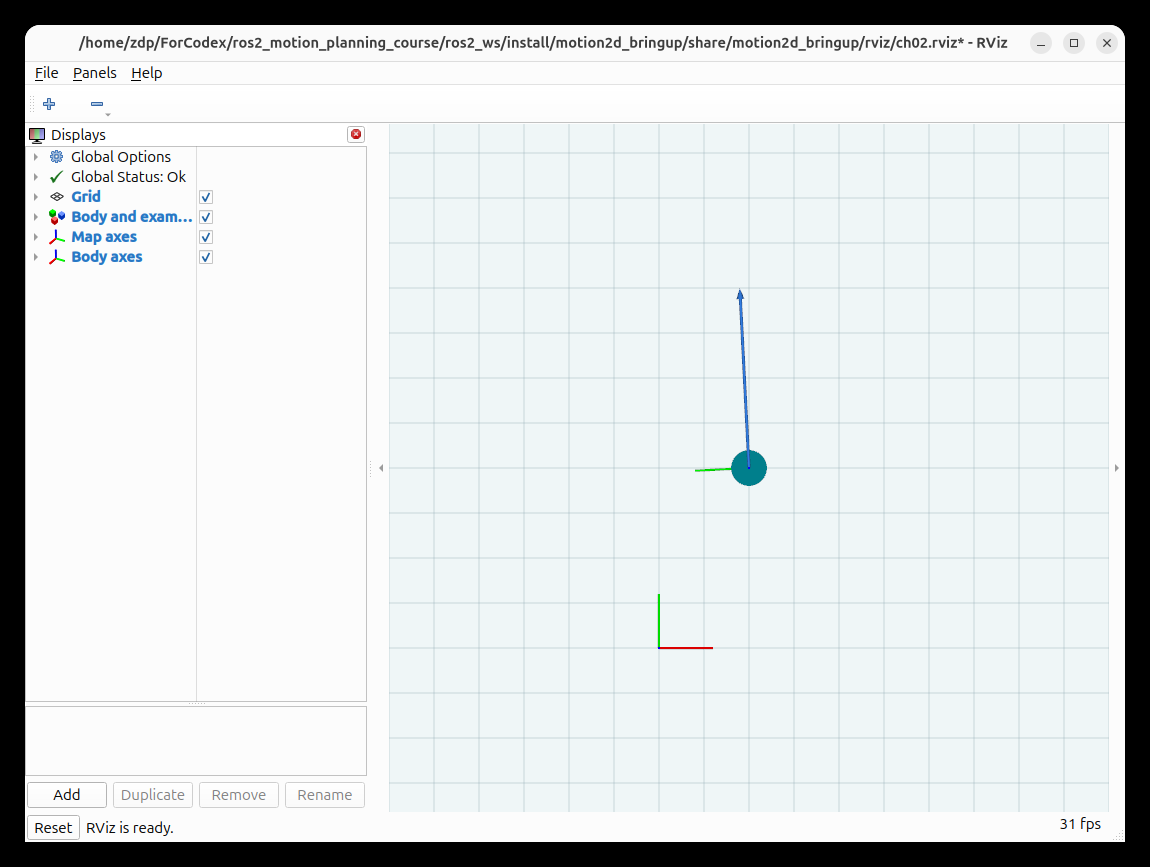
\includegraphics[width=.65\linewidth]{figures/ch02_rviz.png}
\caption{圆心保持在 $(1,2)$，蓝色观测向量随机体坐标系转动；地图坐标轴保持不动。}
\end{figure}

\subsection*{时间练习}
先暂停，再连续调用 step 十次，预测仿真时间增量和朝向增量，之后查看 \code{/clock} 和 TF 核对。标准答案是 0.05 s 与 0.01 rad。改变 YAML 中的 dt 后要重新推导；不应继续照搬默认值的检查脚本。

